% How a training label is made for one PR (see docs/context_selector_roadmap.md 8.5 and 9.3).
% Generated by a script. Token counts are the real per-level input tokens of
% FreeCAD/FreeCAD#21257; findings, coverage and scores are made up for illustration.
% Build: latexmk -pdf selector_training.tex
\documentclass[tikz,border=4pt]{standalone}
\usepackage[T1]{fontenc}
\usepackage[default]{sourcesanspro}
\usepackage{amsmath,amssymb}
\usepackage{fontawesome5}
\usetikzlibrary{calc,arrows.meta,positioning}

\definecolor{ink}{HTML}{1F2328}   \definecolor{grey}{HTML}{6E6A65}  \definecolor{hair}{HTML}{DEDAD4}
\definecolor{inS}{HTML}{5C5751}   \definecolor{inF}{HTML}{FAF9F7}
\definecolor{ourS}{HTML}{2E7D78}  \definecolor{ourF}{HTML}{EDF6F5}  \definecolor{ourD}{HTML}{1F5E5A}
\definecolor{ourB}{HTML}{B5D8D4}
\definecolor{llmS}{HTML}{4F5D8C}  \definecolor{llmF}{HTML}{F1F2F8}
\definecolor{judS}{HTML}{8A6A2F}  \definecolor{judF}{HTML}{FBF7EE}
\definecolor{accC}{HTML}{E06A4E}

\tikzset{
  >={Latex[length=2.6mm,width=2.1mm]},
  column/.style 2 args={draw=#1, fill=#2, line width=0.9pt, rounded corners=8pt},
  title/.style={font=\large\bfseries, anchor=north west, inner sep=0pt},
  step/.style={circle, fill=#1, text=white, font=\small\bfseries, inner sep=0pt, minimum size=0.55cm},
  body/.style={font=\scriptsize, text=grey, anchor=north west, inner sep=0pt, align=left},
  main/.style={->, line width=1.5pt, draw=ink},
}

\begin{document}
\begin{tikzpicture}
\def\top{0}\def\bot{-7.3}

% ======================================================================== columns
\draw[column={inS}{inF}]   (0,\top) rectangle (5.6,\bot);
\draw[column={llmS}{llmF}] (6.3,\top) rectangle (10.9,\bot);
\draw[column={judS}{judF}] (11.6,\top) rectangle (16.3,\bot);
\draw[column={ourS}{ourF}] (17.0,\top) rectangle (23.35,\bot);

\node[step=inS]  at (0.55,-0.6) {1};  \node[title, text=inS, anchor=base west] at (1.0,-0.78) {Ten contexts of one PR};
\node[step=llmS] at (6.85,-0.6) {2};  \node[title, text=llmS, anchor=base west] at (7.3,-0.78) {Frozen LLM};
\node[step=judS] at (12.15,-0.6) {3}; \node[title, text=judS, anchor=base west] at (12.6,-0.78) {AACR judge};
\node[step=ourS] at (17.55,-0.6) {4}; \node[title, text=ourD, anchor=base west] at (18.0,-0.78) {Training label};

\node[body, text width=5.0cm] at (0.3,-1.1) {FreeCAD \#21257 ``Fix hole centered on point edge case''; input tokens of each level};
\node[body, text width=4.2cm] at (6.6,-1.1) {{\color{llmS}\faSnowflake}\; Qwen3.8-27B reviews each level once; chips = generated findings};
\node[body, text width=4.4cm] at (11.9,-1.1) {which of the 6 human comments each review found};
\node[body, text width=6.0cm] at (17.3,-1.1) {score = quality $-\ \lambda\cdot$tokens\,/\,tokens$_{\max}$ \;(here quality = recall, $\lambda=0.5$); the best level is the answer};

% column sub-headers
\node[font=\scriptsize\bfseries, text=ink, anchor=west] at (2.05,-2.25) {tokens};
\node[font=\scriptsize\bfseries, text=ink, anchor=west] at (7.0,-2.25) {findings};
\foreach \j in {1,...,6}{\node[font=\scriptsize\bfseries, text=ink] at ({12.15+0.42*(\j-1)},-2.25) {R\j};}
\node[font=\scriptsize\bfseries, text=ink, anchor=west] at (14.75,-2.25) {recall};
\node[font=\scriptsize\bfseries, text=ink, anchor=west] at (17.75,-2.25) {score};

\node[font=\scriptsize, text=ink, anchor=east, inner sep=0pt] at (1.95,-2.750) {L01 diff};
\fill[ourB, rounded corners=1pt] (2.05,-2.840) rectangle ++(0.102,0.18);
\node[font=\scriptsize, text=grey, anchor=west, inner sep=2pt] at (2.152,-2.750) {13k};
\fill[llmS!55, rounded corners=1pt] (7.000,-2.850) rectangle ++(0.29,0.2);
\fill[white] (7.040,-2.730) rectangle ++(0.2,0.035);
\fill[llmS!55, rounded corners=1pt] (7.360,-2.850) rectangle ++(0.29,0.2);
\fill[white] (7.400,-2.730) rectangle ++(0.2,0.035);
\node[font=\scriptsize, text=grey, anchor=west] at (7.720,-2.750) {2};
\fill[ourS] (12.150,-2.750) circle (0.12);
\node[text=white, font=\tiny] at (12.150,-2.750) {\faCheck};
\draw[hair!80!grey, line width=0.8pt] (12.570,-2.750) circle (0.115);
\draw[hair!80!grey, line width=0.8pt] (12.990,-2.750) circle (0.115);
\draw[hair!80!grey, line width=0.8pt] (13.410,-2.750) circle (0.115);
\draw[hair!80!grey, line width=0.8pt] (13.830,-2.750) circle (0.115);
\draw[hair!80!grey, line width=0.8pt] (14.250,-2.750) circle (0.115);
\node[font=\scriptsize, text=ink, anchor=west] at (14.75,-2.750) {1/6};
\fill[ourS!45, rounded corners=1pt] (17.75,-2.840) rectangle ++(0.508,0.18);
\node[font=\scriptsize, text=grey, anchor=west, inner sep=2pt] at (18.258,-2.750) {0.14};
\node[font=\scriptsize, text=ink, anchor=east, inner sep=0pt] at (1.95,-3.220) {L02 + functions};
\fill[ourB, rounded corners=1pt] (2.05,-3.310) rectangle ++(0.319,0.18);
\node[font=\scriptsize, text=grey, anchor=west, inner sep=2pt] at (2.369,-3.220) {41k};
\fill[llmS!55, rounded corners=1pt] (7.000,-3.320) rectangle ++(0.29,0.2);
\fill[white] (7.040,-3.200) rectangle ++(0.2,0.035);
\fill[llmS!55, rounded corners=1pt] (7.360,-3.320) rectangle ++(0.29,0.2);
\fill[white] (7.400,-3.200) rectangle ++(0.2,0.035);
\fill[llmS!55, rounded corners=1pt] (7.720,-3.320) rectangle ++(0.29,0.2);
\fill[white] (7.760,-3.200) rectangle ++(0.2,0.035);
\node[font=\scriptsize, text=grey, anchor=west] at (8.080,-3.220) {3};
\fill[ourS] (12.150,-3.220) circle (0.12);
\node[text=white, font=\tiny] at (12.150,-3.220) {\faCheck};
\draw[hair!80!grey, line width=0.8pt] (12.570,-3.220) circle (0.115);
\draw[hair!80!grey, line width=0.8pt] (12.990,-3.220) circle (0.115);
\fill[ourS] (13.410,-3.220) circle (0.12);
\node[text=white, font=\tiny] at (13.410,-3.220) {\faCheck};
\draw[hair!80!grey, line width=0.8pt] (13.830,-3.220) circle (0.115);
\draw[hair!80!grey, line width=0.8pt] (14.250,-3.220) circle (0.115);
\node[font=\scriptsize, text=ink, anchor=west] at (14.75,-3.220) {2/6};
\fill[ourS!45, rounded corners=1pt] (17.75,-3.310) rectangle ++(0.913,0.18);
\node[font=\scriptsize, text=grey, anchor=west, inner sep=2pt] at (18.663,-3.220) {0.25};
\node[font=\scriptsize, text=ink, anchor=east, inner sep=0pt] at (1.95,-3.690) {L03 + files};
\fill[ourB, rounded corners=1pt] (2.05,-3.780) rectangle ++(0.500,0.18);
\node[font=\scriptsize, text=grey, anchor=west, inner sep=2pt] at (2.550,-3.690) {64k};
\fill[llmS!55, rounded corners=1pt] (7.000,-3.790) rectangle ++(0.29,0.2);
\fill[white] (7.040,-3.670) rectangle ++(0.2,0.035);
\fill[llmS!55, rounded corners=1pt] (7.360,-3.790) rectangle ++(0.29,0.2);
\fill[white] (7.400,-3.670) rectangle ++(0.2,0.035);
\fill[llmS!55, rounded corners=1pt] (7.720,-3.790) rectangle ++(0.29,0.2);
\fill[white] (7.760,-3.670) rectangle ++(0.2,0.035);
\node[font=\scriptsize, text=grey, anchor=west] at (8.080,-3.690) {3};
\fill[ourS] (12.150,-3.690) circle (0.12);
\node[text=white, font=\tiny] at (12.150,-3.690) {\faCheck};
\fill[ourS] (12.570,-3.690) circle (0.12);
\node[text=white, font=\tiny] at (12.570,-3.690) {\faCheck};
\draw[hair!80!grey, line width=0.8pt] (12.990,-3.690) circle (0.115);
\fill[ourS] (13.410,-3.690) circle (0.12);
\node[text=white, font=\tiny] at (13.410,-3.690) {\faCheck};
\draw[hair!80!grey, line width=0.8pt] (13.830,-3.690) circle (0.115);
\draw[hair!80!grey, line width=0.8pt] (14.250,-3.690) circle (0.115);
\node[font=\scriptsize, text=ink, anchor=west] at (14.75,-3.690) {3/6};
\fill[ourS!45, rounded corners=1pt] (17.75,-3.780) rectangle ++(1.350,0.18);
\node[font=\scriptsize, text=grey, anchor=west, inner sep=2pt] at (19.100,-3.690) {0.37};
\fill[accC!10, rounded corners=3pt] (0.25,-4.370) rectangle (23.1,-3.950);
\node[font=\scriptsize\bfseries, text=accC, anchor=east, inner sep=0pt] at (1.95,-4.160) {L04 + callees};
\fill[accC, rounded corners=1pt] (2.05,-4.250) rectangle ++(0.610,0.18);
\node[font=\scriptsize\bfseries, text=accC, anchor=west, inner sep=2pt] at (2.660,-4.160) {78k};
\fill[llmS!55, rounded corners=1pt] (7.000,-4.260) rectangle ++(0.29,0.2);
\fill[white] (7.040,-4.140) rectangle ++(0.2,0.035);
\fill[llmS!55, rounded corners=1pt] (7.360,-4.260) rectangle ++(0.29,0.2);
\fill[white] (7.400,-4.140) rectangle ++(0.2,0.035);
\fill[llmS!55, rounded corners=1pt] (7.720,-4.260) rectangle ++(0.29,0.2);
\fill[white] (7.760,-4.140) rectangle ++(0.2,0.035);
\fill[llmS!55, rounded corners=1pt] (8.080,-4.260) rectangle ++(0.29,0.2);
\fill[white] (8.120,-4.140) rectangle ++(0.2,0.035);
\node[font=\scriptsize, text=grey, anchor=west] at (8.440,-4.160) {4};
\fill[ourS] (12.150,-4.160) circle (0.12);
\node[text=white, font=\tiny] at (12.150,-4.160) {\faCheck};
\fill[ourS] (12.570,-4.160) circle (0.12);
\node[text=white, font=\tiny] at (12.570,-4.160) {\faCheck};
\fill[ourS] (12.990,-4.160) circle (0.12);
\node[text=white, font=\tiny] at (12.990,-4.160) {\faCheck};
\fill[ourS] (13.410,-4.160) circle (0.12);
\node[text=white, font=\tiny] at (13.410,-4.160) {\faCheck};
\draw[hair!80!grey, line width=0.8pt] (13.830,-4.160) circle (0.115);
\draw[hair!80!grey, line width=0.8pt] (14.250,-4.160) circle (0.115);
\node[font=\scriptsize\bfseries, text=accC, anchor=west] at (14.75,-4.160) {4/6};
\fill[accC, rounded corners=1pt] (17.75,-4.250) rectangle ++(1.851,0.18);
\node[font=\scriptsize\bfseries, text=accC, anchor=west, inner sep=2pt] at (19.601,-4.160) {0.51};
\node[font=\scriptsize, text=ink, anchor=east, inner sep=0pt] at (1.95,-4.630) {L05 + callers};
\fill[ourB, rounded corners=1pt] (2.05,-4.720) rectangle ++(0.678,0.18);
\node[font=\scriptsize, text=grey, anchor=west, inner sep=2pt] at (2.728,-4.630) {87k};
\fill[llmS!55, rounded corners=1pt] (7.000,-4.730) rectangle ++(0.29,0.2);
\fill[white] (7.040,-4.610) rectangle ++(0.2,0.035);
\fill[llmS!55, rounded corners=1pt] (7.360,-4.730) rectangle ++(0.29,0.2);
\fill[white] (7.400,-4.610) rectangle ++(0.2,0.035);
\fill[llmS!55, rounded corners=1pt] (7.720,-4.730) rectangle ++(0.29,0.2);
\fill[white] (7.760,-4.610) rectangle ++(0.2,0.035);
\fill[llmS!55, rounded corners=1pt] (8.080,-4.730) rectangle ++(0.29,0.2);
\fill[white] (8.120,-4.610) rectangle ++(0.2,0.035);
\node[font=\scriptsize, text=grey, anchor=west] at (8.440,-4.630) {4};
\fill[ourS] (12.150,-4.630) circle (0.12);
\node[text=white, font=\tiny] at (12.150,-4.630) {\faCheck};
\fill[ourS] (12.570,-4.630) circle (0.12);
\node[text=white, font=\tiny] at (12.570,-4.630) {\faCheck};
\fill[ourS] (12.990,-4.630) circle (0.12);
\node[text=white, font=\tiny] at (12.990,-4.630) {\faCheck};
\fill[ourS] (13.410,-4.630) circle (0.12);
\node[text=white, font=\tiny] at (13.410,-4.630) {\faCheck};
\draw[hair!80!grey, line width=0.8pt] (13.830,-4.630) circle (0.115);
\draw[hair!80!grey, line width=0.8pt] (14.250,-4.630) circle (0.115);
\node[font=\scriptsize, text=ink, anchor=west] at (14.75,-4.630) {4/6};
\fill[ourS!45, rounded corners=1pt] (17.75,-4.720) rectangle ++(1.790,0.18);
\node[font=\scriptsize, text=grey, anchor=west, inner sep=2pt] at (19.540,-4.630) {0.50};
\node[font=\scriptsize, text=ink, anchor=east, inner sep=0pt] at (1.95,-5.100) {L06 + tests};
\fill[ourB, rounded corners=1pt] (2.05,-5.190) rectangle ++(0.678,0.18);
\node[font=\scriptsize, text=grey, anchor=west, inner sep=2pt] at (2.728,-5.100) {87k};
\fill[llmS!55, rounded corners=1pt] (7.000,-5.200) rectangle ++(0.29,0.2);
\fill[white] (7.040,-5.080) rectangle ++(0.2,0.035);
\fill[llmS!55, rounded corners=1pt] (7.360,-5.200) rectangle ++(0.29,0.2);
\fill[white] (7.400,-5.080) rectangle ++(0.2,0.035);
\fill[llmS!55, rounded corners=1pt] (7.720,-5.200) rectangle ++(0.29,0.2);
\fill[white] (7.760,-5.080) rectangle ++(0.2,0.035);
\fill[llmS!55, rounded corners=1pt] (8.080,-5.200) rectangle ++(0.29,0.2);
\fill[white] (8.120,-5.080) rectangle ++(0.2,0.035);
\node[font=\scriptsize, text=grey, anchor=west] at (8.440,-5.100) {4};
\fill[ourS] (12.150,-5.100) circle (0.12);
\node[text=white, font=\tiny] at (12.150,-5.100) {\faCheck};
\fill[ourS] (12.570,-5.100) circle (0.12);
\node[text=white, font=\tiny] at (12.570,-5.100) {\faCheck};
\fill[ourS] (12.990,-5.100) circle (0.12);
\node[text=white, font=\tiny] at (12.990,-5.100) {\faCheck};
\fill[ourS] (13.410,-5.100) circle (0.12);
\node[text=white, font=\tiny] at (13.410,-5.100) {\faCheck};
\draw[hair!80!grey, line width=0.8pt] (13.830,-5.100) circle (0.115);
\draw[hair!80!grey, line width=0.8pt] (14.250,-5.100) circle (0.115);
\node[font=\scriptsize, text=ink, anchor=west] at (14.75,-5.100) {4/6};
\fill[ourS!45, rounded corners=1pt] (17.75,-5.190) rectangle ++(1.790,0.18);
\node[font=\scriptsize, text=grey, anchor=west, inner sep=2pt] at (19.540,-5.100) {0.50};
\node[font=\scriptsize, text=ink, anchor=east, inner sep=0pt] at (1.95,-5.570) {L07 + guides};
\fill[ourB, rounded corners=1pt] (2.05,-5.660) rectangle ++(0.711,0.18);
\node[font=\scriptsize, text=grey, anchor=west, inner sep=2pt] at (2.761,-5.570) {91k};
\fill[llmS!55, rounded corners=1pt] (7.000,-5.670) rectangle ++(0.29,0.2);
\fill[white] (7.040,-5.550) rectangle ++(0.2,0.035);
\fill[llmS!55, rounded corners=1pt] (7.360,-5.670) rectangle ++(0.29,0.2);
\fill[white] (7.400,-5.550) rectangle ++(0.2,0.035);
\fill[llmS!55, rounded corners=1pt] (7.720,-5.670) rectangle ++(0.29,0.2);
\fill[white] (7.760,-5.550) rectangle ++(0.2,0.035);
\fill[llmS!55, rounded corners=1pt] (8.080,-5.670) rectangle ++(0.29,0.2);
\fill[white] (8.120,-5.550) rectangle ++(0.2,0.035);
\fill[llmS!55, rounded corners=1pt] (8.440,-5.670) rectangle ++(0.29,0.2);
\fill[white] (8.480,-5.550) rectangle ++(0.2,0.035);
\node[font=\scriptsize, text=grey, anchor=west] at (8.800,-5.570) {5};
\fill[ourS] (12.150,-5.570) circle (0.12);
\node[text=white, font=\tiny] at (12.150,-5.570) {\faCheck};
\fill[ourS] (12.570,-5.570) circle (0.12);
\node[text=white, font=\tiny] at (12.570,-5.570) {\faCheck};
\fill[ourS] (12.990,-5.570) circle (0.12);
\node[text=white, font=\tiny] at (12.990,-5.570) {\faCheck};
\fill[ourS] (13.410,-5.570) circle (0.12);
\node[text=white, font=\tiny] at (13.410,-5.570) {\faCheck};
\draw[hair!80!grey, line width=0.8pt] (13.830,-5.570) circle (0.115);
\draw[hair!80!grey, line width=0.8pt] (14.250,-5.570) circle (0.115);
\node[font=\scriptsize, text=ink, anchor=west] at (14.75,-5.570) {4/6};
\fill[ourS!45, rounded corners=1pt] (17.75,-5.660) rectangle ++(1.760,0.18);
\node[font=\scriptsize, text=grey, anchor=west, inner sep=2pt] at (19.510,-5.570) {0.49};
\node[font=\scriptsize, text=ink, anchor=east, inner sep=0pt] at (1.95,-6.040) {L08 2 hops};
\fill[ourB, rounded corners=1pt] (2.05,-6.130) rectangle ++(0.923,0.18);
\node[font=\scriptsize, text=grey, anchor=west, inner sep=2pt] at (2.973,-6.040) {118k};
\fill[llmS!55, rounded corners=1pt] (7.000,-6.140) rectangle ++(0.29,0.2);
\fill[white] (7.040,-6.020) rectangle ++(0.2,0.035);
\fill[llmS!55, rounded corners=1pt] (7.360,-6.140) rectangle ++(0.29,0.2);
\fill[white] (7.400,-6.020) rectangle ++(0.2,0.035);
\fill[llmS!55, rounded corners=1pt] (7.720,-6.140) rectangle ++(0.29,0.2);
\fill[white] (7.760,-6.020) rectangle ++(0.2,0.035);
\fill[llmS!55, rounded corners=1pt] (8.080,-6.140) rectangle ++(0.29,0.2);
\fill[white] (8.120,-6.020) rectangle ++(0.2,0.035);
\fill[llmS!55, rounded corners=1pt] (8.440,-6.140) rectangle ++(0.29,0.2);
\fill[white] (8.480,-6.020) rectangle ++(0.2,0.035);
\node[font=\scriptsize, text=grey, anchor=west] at (8.800,-6.040) {5};
\fill[ourS] (12.150,-6.040) circle (0.12);
\node[text=white, font=\tiny] at (12.150,-6.040) {\faCheck};
\fill[ourS] (12.570,-6.040) circle (0.12);
\node[text=white, font=\tiny] at (12.570,-6.040) {\faCheck};
\draw[hair!80!grey, line width=0.8pt] (12.990,-6.040) circle (0.115);
\fill[ourS] (13.410,-6.040) circle (0.12);
\node[text=white, font=\tiny] at (13.410,-6.040) {\faCheck};
\fill[ourS] (13.830,-6.040) circle (0.12);
\node[text=white, font=\tiny] at (13.830,-6.040) {\faCheck};
\draw[hair!80!grey, line width=0.8pt] (14.250,-6.040) circle (0.115);
\node[font=\scriptsize, text=ink, anchor=west] at (14.75,-6.040) {4/6};
\fill[ourS!45, rounded corners=1pt] (17.75,-6.130) rectangle ++(1.569,0.18);
\node[font=\scriptsize, text=grey, anchor=west, inner sep=2pt] at (19.319,-6.040) {0.44};
\node[font=\scriptsize, text=ink, anchor=east, inner sep=0pt] at (1.95,-6.510) {L09 + docs};
\fill[ourB, rounded corners=1pt] (2.05,-6.600) rectangle ++(0.925,0.18);
\node[font=\scriptsize, text=grey, anchor=west, inner sep=2pt] at (2.975,-6.510) {119k};
\fill[llmS!55, rounded corners=1pt] (7.000,-6.610) rectangle ++(0.29,0.2);
\fill[white] (7.040,-6.490) rectangle ++(0.2,0.035);
\fill[llmS!55, rounded corners=1pt] (7.360,-6.610) rectangle ++(0.29,0.2);
\fill[white] (7.400,-6.490) rectangle ++(0.2,0.035);
\fill[llmS!55, rounded corners=1pt] (7.720,-6.610) rectangle ++(0.29,0.2);
\fill[white] (7.760,-6.490) rectangle ++(0.2,0.035);
\fill[llmS!55, rounded corners=1pt] (8.080,-6.610) rectangle ++(0.29,0.2);
\fill[white] (8.120,-6.490) rectangle ++(0.2,0.035);
\fill[llmS!55, rounded corners=1pt] (8.440,-6.610) rectangle ++(0.29,0.2);
\fill[white] (8.480,-6.490) rectangle ++(0.2,0.035);
\fill[llmS!55, rounded corners=1pt] (8.800,-6.610) rectangle ++(0.29,0.2);
\fill[white] (8.840,-6.490) rectangle ++(0.2,0.035);
\node[font=\scriptsize, text=grey, anchor=west] at (9.160,-6.510) {6};
\fill[ourS] (12.150,-6.510) circle (0.12);
\node[text=white, font=\tiny] at (12.150,-6.510) {\faCheck};
\fill[ourS] (12.570,-6.510) circle (0.12);
\node[text=white, font=\tiny] at (12.570,-6.510) {\faCheck};
\fill[ourS] (12.990,-6.510) circle (0.12);
\node[text=white, font=\tiny] at (12.990,-6.510) {\faCheck};
\fill[ourS] (13.410,-6.510) circle (0.12);
\node[text=white, font=\tiny] at (13.410,-6.510) {\faCheck};
\draw[hair!80!grey, line width=0.8pt] (13.830,-6.510) circle (0.115);
\draw[hair!80!grey, line width=0.8pt] (14.250,-6.510) circle (0.115);
\node[font=\scriptsize, text=ink, anchor=west] at (14.75,-6.510) {4/6};
\fill[ourS!45, rounded corners=1pt] (17.75,-6.600) rectangle ++(1.567,0.18);
\node[font=\scriptsize, text=grey, anchor=west, inner sep=2pt] at (19.317,-6.510) {0.44};
\node[font=\scriptsize, text=ink, anchor=east, inner sep=0pt] at (1.95,-6.980) {L10 all};
\fill[ourB, rounded corners=1pt] (2.05,-7.070) rectangle ++(2.000,0.18);
\node[font=\scriptsize, text=grey, anchor=west, inner sep=2pt] at (4.050,-6.980) {256k};
\fill[llmS!55, rounded corners=1pt] (7.000,-7.080) rectangle ++(0.29,0.2);
\fill[white] (7.040,-6.960) rectangle ++(0.2,0.035);
\fill[llmS!55, rounded corners=1pt] (7.360,-7.080) rectangle ++(0.29,0.2);
\fill[white] (7.400,-6.960) rectangle ++(0.2,0.035);
\fill[llmS!55, rounded corners=1pt] (7.720,-7.080) rectangle ++(0.29,0.2);
\fill[white] (7.760,-6.960) rectangle ++(0.2,0.035);
\fill[llmS!55, rounded corners=1pt] (8.080,-7.080) rectangle ++(0.29,0.2);
\fill[white] (8.120,-6.960) rectangle ++(0.2,0.035);
\fill[llmS!55, rounded corners=1pt] (8.440,-7.080) rectangle ++(0.29,0.2);
\fill[white] (8.480,-6.960) rectangle ++(0.2,0.035);
\fill[llmS!55, rounded corners=1pt] (8.800,-7.080) rectangle ++(0.29,0.2);
\fill[white] (8.840,-6.960) rectangle ++(0.2,0.035);
\node[font=\scriptsize, text=grey, anchor=west] at (9.160,-6.980) {6};
\fill[ourS] (12.150,-6.980) circle (0.12);
\node[text=white, font=\tiny] at (12.150,-6.980) {\faCheck};
\fill[ourS] (12.570,-6.980) circle (0.12);
\node[text=white, font=\tiny] at (12.570,-6.980) {\faCheck};
\fill[ourS] (12.990,-6.980) circle (0.12);
\node[text=white, font=\tiny] at (12.990,-6.980) {\faCheck};
\fill[ourS] (13.410,-6.980) circle (0.12);
\node[text=white, font=\tiny] at (13.410,-6.980) {\faCheck};
\fill[ourS] (13.830,-6.980) circle (0.12);
\node[text=white, font=\tiny] at (13.830,-6.980) {\faCheck};
\draw[hair!80!grey, line width=0.8pt] (14.250,-6.980) circle (0.115);
\node[font=\scriptsize, text=ink, anchor=west] at (14.75,-6.980) {5/6};
\fill[ourS!45, rounded corners=1pt] (17.75,-7.070) rectangle ++(1.200,0.18);
\node[font=\scriptsize, text=grey, anchor=west, inner sep=2pt] at (18.950,-6.980) {0.33};

% ======================================================================== label call-out
\node[draw=accC, fill=white, line width=1.1pt, rounded corners=5pt, align=center, font=\small, inner sep=5pt,
      anchor=west] (lab) at (21.2,-4.160) {\textbf{\color{accC}label}\\ $y=$ \textbf{L04}};

% arrows between columns
\foreach \x in {5.6,10.9,16.3}{\draw[main] (\x+0.02,-0.6) -- (\x+0.68,-0.6);}
\node[font=\small, text=ink, anchor=north west, inner sep=0pt] at (0.1,-7.55) {Repeated for all 196 PRs: an outcome table of 1,960 reviews, built once. The selector then learns input-side features $\mathbf{x}\mapsto$ label $y$ by table lookup, without calling the LLM.};
\node[font=\scriptsize\itshape, text=grey, anchor=north east, inner sep=0pt] at (23.35,-8.05) {findings, coverage and scores are illustrative};

\end{tikzpicture}
\end{document}
